% \documentclass[sigconf]{acmart}
\documentclass[sigconf, review]{acmart}
%%
%% \BibTeX command to typeset BibTeX logo in the docs
\AtBeginDocument{%https://www.overleaf.com/project
  \providecommand\BibTeX{{%
    Bib\TeX}}}

%% Rights management information.  This information is sent to you
%% when you complete the rights form.  These commands have SAMPLE
%% values in them; it is your responsibility as an author to replace
%% the commands and values with those provided to you when you
%% complete the rights form.
\setcopyright{acmlicensed}
\copyrightyear{2018}
\acmYear{2018}
\acmDOI{XXXXXXX.XXXXXXX}
%% These commands are for a PROCEEDINGS abstract or paper.
% \acmConference[Conference acronym 'XX]{Make sure to enter the correct
%   conference title from your rights confirmation email}{June 03--05,
%   2018}{Woodstock, NY}
%%
%%  Uncomment \acmBooktitle if the title of the proceedings is different
%%  from ``Proceedings of ...''!
%%
%%\acmBooktitle{Woodstock '18: ACM Symposium on Neural Gaze Detection,
%%  June 03--05, 2018, Woodstock, NY}
\acmISBN{978-1-4503-XXXX-X/2018/06}



\begin{document}

%%
%% The "title" command has an optional parameter,
%% allowing the author to define a "short title" to be used in page headers.
\title{Generative Flow-Matching Modeling of the Neurodevelopmental Connectome via Dynamic Hypergraphs}

%%
%% The "author" command and its associated commands are used to define
%% the authors and their affiliations.
%% Of note is the shared affiliation of the first two authors, and the
%% "authornote" and "authornotemark" commands
%% used to denote shared contribution to the research.
\author{Katherine Birch}
% \authornote{Both authors contributed equally to this research.}
\email{k.birch@surrey.ac.uk}
\orcid{}
% \author{G.K.M. Tobin}
% \authornotemark[1]
% \email{webmaster@marysville-ohio.com}
\affiliation{%
  \institution{NICE Research Group, Computer Science Research Centre, School of Computer Science and Electronic Engineering, University of Surrey}
  \city{Guildford}
  \country{United Kingdom}
}

 

\author{Alberto Durán-López}
\affiliation{%
  \institution{Research Centre for Information and Communication Technologies (CITIC-UGR), University of Granada}
  \city{Granada}
  \country{Spain}}
% \email{albduranlopez@ugr.es}

\author{Daniel Bolaños-Martinez}
\affiliation{%
  \institution{Research Centre for Information and Communication Technologies (CITIC-UGR), University of Granada}
  \city{Granada}
  \country{Spain}}
% \email{danibolanos@ugr.es}

\author{Maria Bermudez-Edo}
\affiliation{%
  \institution{Research Centre for Information and Communication Technologies (CITIC-UGR), University of Granada}
  \city{Granada}
  \country{Spain}}
 % \email{mbe@ugr.es}


 \author{Roman Bauer}
\affiliation{%
  \institution{NICE Research Group, Computer Science Research Centre, School of Computer Science and Electronic Engineering, University of Surrey}
  \city{Guildford}
  \country{United Kingdom}
}


\author{Suparna De}
\affiliation{%
  \institution{NICE Research Group, Computer Science Research Centre, School of Computer Science and Electronic Engineering, University of Surrey}
  \city{Guildford}
  \country{United Kingdom}
  \email{s.de@surrey.ac.uk}
}


%%
%% By default, the full list of authors will be used in the page
%% headers. Often, this list is too long, and will overlap
%% other information printed in the page headers. This command allows
%% the author to define a more concise list
%% of authors' names for this purpose.
% \renewcommand{\shortauthors}{Trovato et al.}


\begin{abstract}


% biologically aware conditional graph diffusion model
% preterm birth
% brain connectivity pattern
% small datasets
% hypergraph information integration
Human brain structure datasets are regularly small and lack a representative sample of target phenotypes. Augmenting these is often challenging due to highly complex patterns of connectivity, and this issue is particularly emphasized when there are significant target class imbalances. We introduce a model that enables the generation of novel data instances and data exploration. Specifically, we consider the case of preterm birth, where datasets include very few preterm individuals. We present a diffusion-style flow-matching framework, whereby conditioning on continuous gestational age (GA), the model learns the underlying geometry of the brain and can reproduce differences in connectivities for infants born at varying numbers of weeks. This approach is inspired by the brain's fundamental capacity for self-organization. Moreover, to understand the real implications of varying GA on the organization of the developing brain, we integrate a dynamic hypergraph layer. This allows the model to dynamically learn the higher-order dependencies that evolve in the brain, facilitating the generation of biologically plausible structural topologies. To ensure appropriateness and sufficiency in the generated networks, we utilize biologically inspired losses. Additionally, we compare the generation with key graph metrics commonly employed in neurobiological studies of brain structure. Our model results demonstrate biologically realistic connectivity patterns discovered through the dynamic hypergraph approach.

\end{abstract}

\keywords{Generative AI, Neuroscience, Hypergraph, Flow matching, Preterm birth}
\maketitle





\section{Introduction}
The human brain undergoes an intensive period of non-linear development during the final stages of pregnancy. This phase is characterized by rapid reinforcement of the brain structures, such as small-world architecture \cite{sporns_human_2013, karolis2016reinforcement} and emergence of structural hubs and global communication \cite{karolis2016reinforcement, ball2012effect, bauer2017nonlinear, taoudi2022predicting}. For infants born prematurely, this developmental trajectory is disrupted. Understanding the divergences between preterm and term born infants at the time of birth can give important insights into group-level differences in complex structures as they emerge \cite{birch2025exploring, schuetze2016morphological, ball2012effect, ream2018neurologic, lee2021cingulum}.  
However, the acquiring data required for these analyses is challenging. The field suffers from consistently small datasets, with low numbers of target phenotypes. This is particularly pronounced when considering the case of infant development due to the high cost of MRI, and the physical difficulty in imaging such small infants \cite{taoudi2022predicting}. This creates a challenge whereby standard models struggle to distinguish between classes, are prone to overfitting and majority class collapse \cite{birch2025exploring, cui2022braingb, messaritaki2019optimization}. To overcome these issues, we propose a generative approach, designed to implicitly learn biological structures from sparse data. Moreover, we propose a model which can learn the implicit latent differences between infants as a function of continuous gestational development. 

We introduce a model that allows generation of novel cases of data, at different gestational ages (GA). We move away from explicitly programmed targets and structural information, through the use of dynamic hyperedge membership, and Conditional Flow Matching.
In summary, we introduce three key contributions:
\begin{enumerate}
    \item We introduce a generative framework capable of interpolating novel data instances across the entire gestational age (GA) window. By conceptualizing neurodevelopment as a continuous trajectory rather than a series of discrete temporal snapshots, the model enables the high-fidelity simulation and exploration of the diverging structural connectomes of preterm and term-born infants.
    \item We demonstrate that the model can produce both biologically plausible and mathematically sufficient connectivity. Using a selection of neurobiological metrics, we provide a validation framework for our synthetic data samples.
    \item Our model proposes a novel integration of Dynamic Hypergraph, with Constrained Flow Matching. By employing a composite, biologically inspired loss function the model implicitly learns higher-order structures and maturation trends.
    
\end{enumerate}
 
\section{Related work}

Traditional methods of generating brain connectivity graphs, used stochastic models guided by explicit, biologically inspired, rules \cite{betzel_generative_2016}. While these are useful for testing assumptions surrounding the mechanism by which brains self-organise, they lack any implicit awareness of gestational age (GA). This means that while they can often reproduce global structures expected from brain graphs, they generate average cases.
More recent work by \citet{liu_deep_2025}, have applied a conditional Variational Autoencoder (CVAE), to model adult brain connectivity optimized for Kullback-Leibler (KL) divergence and reconstruction losses. They successfully reproduce structural connectivity patterns from individual subjects, conditioned on lifestyle and cognitive factors. While this provides a good baseline for generation, the model is reconstructive, learning a mapping for specific individuals within the dataset. This means that the model does not learn to generate novel cases and is prone to struggle on minority classes. Furthermore, in order to overcome data sparsity, they rely on mean imputation for missing GA cases, which may cause oversmoothing of neurodevelopmental trajectories and disruptions. 
Other recent work \cite{xie_controllable_2026} have focused on continuous modeling of the developing brain through diffusion based models. \citet{xie_controllable_2026} introduce a graph-diffusion model that is able to produce realistic simulations of the maturing surface of the brain. Their model is able to rely on standard diffusion models, where iterative denoising steps are able to capture small nuances in surface texture of the brains. Their methodology focuses on high-resolution data, while our problem relies on small datasets, of high-order global structural connectivity. Therefore, we require a model which can ensure stability, while taking advantage of the continuous modeling of gestation from \citet{xie_controllable_2026}.



In order to overcome some of the difficulties faced by traditional diffusion models, Flow Matching has emerged as a powerful alternative. Flow Matching is a deterministic generalization of diffusion, which reduces the computational cost by learning a straight line path between noise and target \cite{lipman2023flowmatchinggenerativemodeling, yan2025trajflow}.  \citet{zhang2024generative} use flow models in social science domain, where specific patterns of connectivity are expected based on prior knowledge. They reward the model based on its ability to achieve certain structural objectives as well as raw data distribution. However, by conditioning on target connectivity patterns, the model is unable to implicitly learn about how those patterns arise.

In order to improve biological realism, \citet{zuo_hemisphere-separated_2023}, used a VAE-GAN architecture which proposed informing the model of structural information regarding which side of the brain each node belongs to. By introducing biological priors, they demonstrate an improvement in Alzheimer's classification on an adult dataset. While this represents a step in biologically aware models, the modeling of hemisphere separation introduces explicit information about the expected connectivity patterns. We can adapt the structural priors to become implicitly aware of developing connectivity structures.  

Moreover, \cite{zuo_hemisphere-separated_2023} these models rely on pairwise regional interactions within the brain. In the early statistical models, graph metrics explored how the brain balances global integration with local communication \cite{sporns_human_2013}. Another study which has shown that the brain is better characterized by higher-order interactions between regions is \citet{xiao_multi-hypergraph_2020}. In their paper, they learn a hypergraph representation of the connectivity matrices, which can discover higher-order interactions between regions. Other researchers have also made use of hypergraph structures for exploring brain functional connectivity \cite{yuan_d-hypernet_2025, sadeghian_hyperbrain_2025, han_hypergraph_2025, han_hypergraph-based_2026}. Functional data generally differs from structural brain connectomes, as it often includes more ROIs, as well as temporal changes within one individual. One study which has applied hypergraph insights to structural brain data was \citet{yuan_d-hypernet_2025}. In their paper, they use hypergraph representations for both functional and structural connectivity, and integrates these hyperedge relationships into a contrastive learning model. While this is a strong model for identifying differences, it lacks the ability to generate novel cases of data, or to simulate the continuous maturation.

The central challenge in generative modeling of brain development is the inability to simulate continuous, higher-order maturation while maintaining individual differences. Existing models suffer from combinations of ``age-blindness'', explicit biological constraints tending models toward prescriptiveness, and difficulty in balancing local and global integration. Therefore, a model that implicitly learns the continuous development of brain structure, while discovering and reproducing complex structures, is highly needed. 


% \subsection{Contributions}



\section{Method}

\begin{figure*}
  % 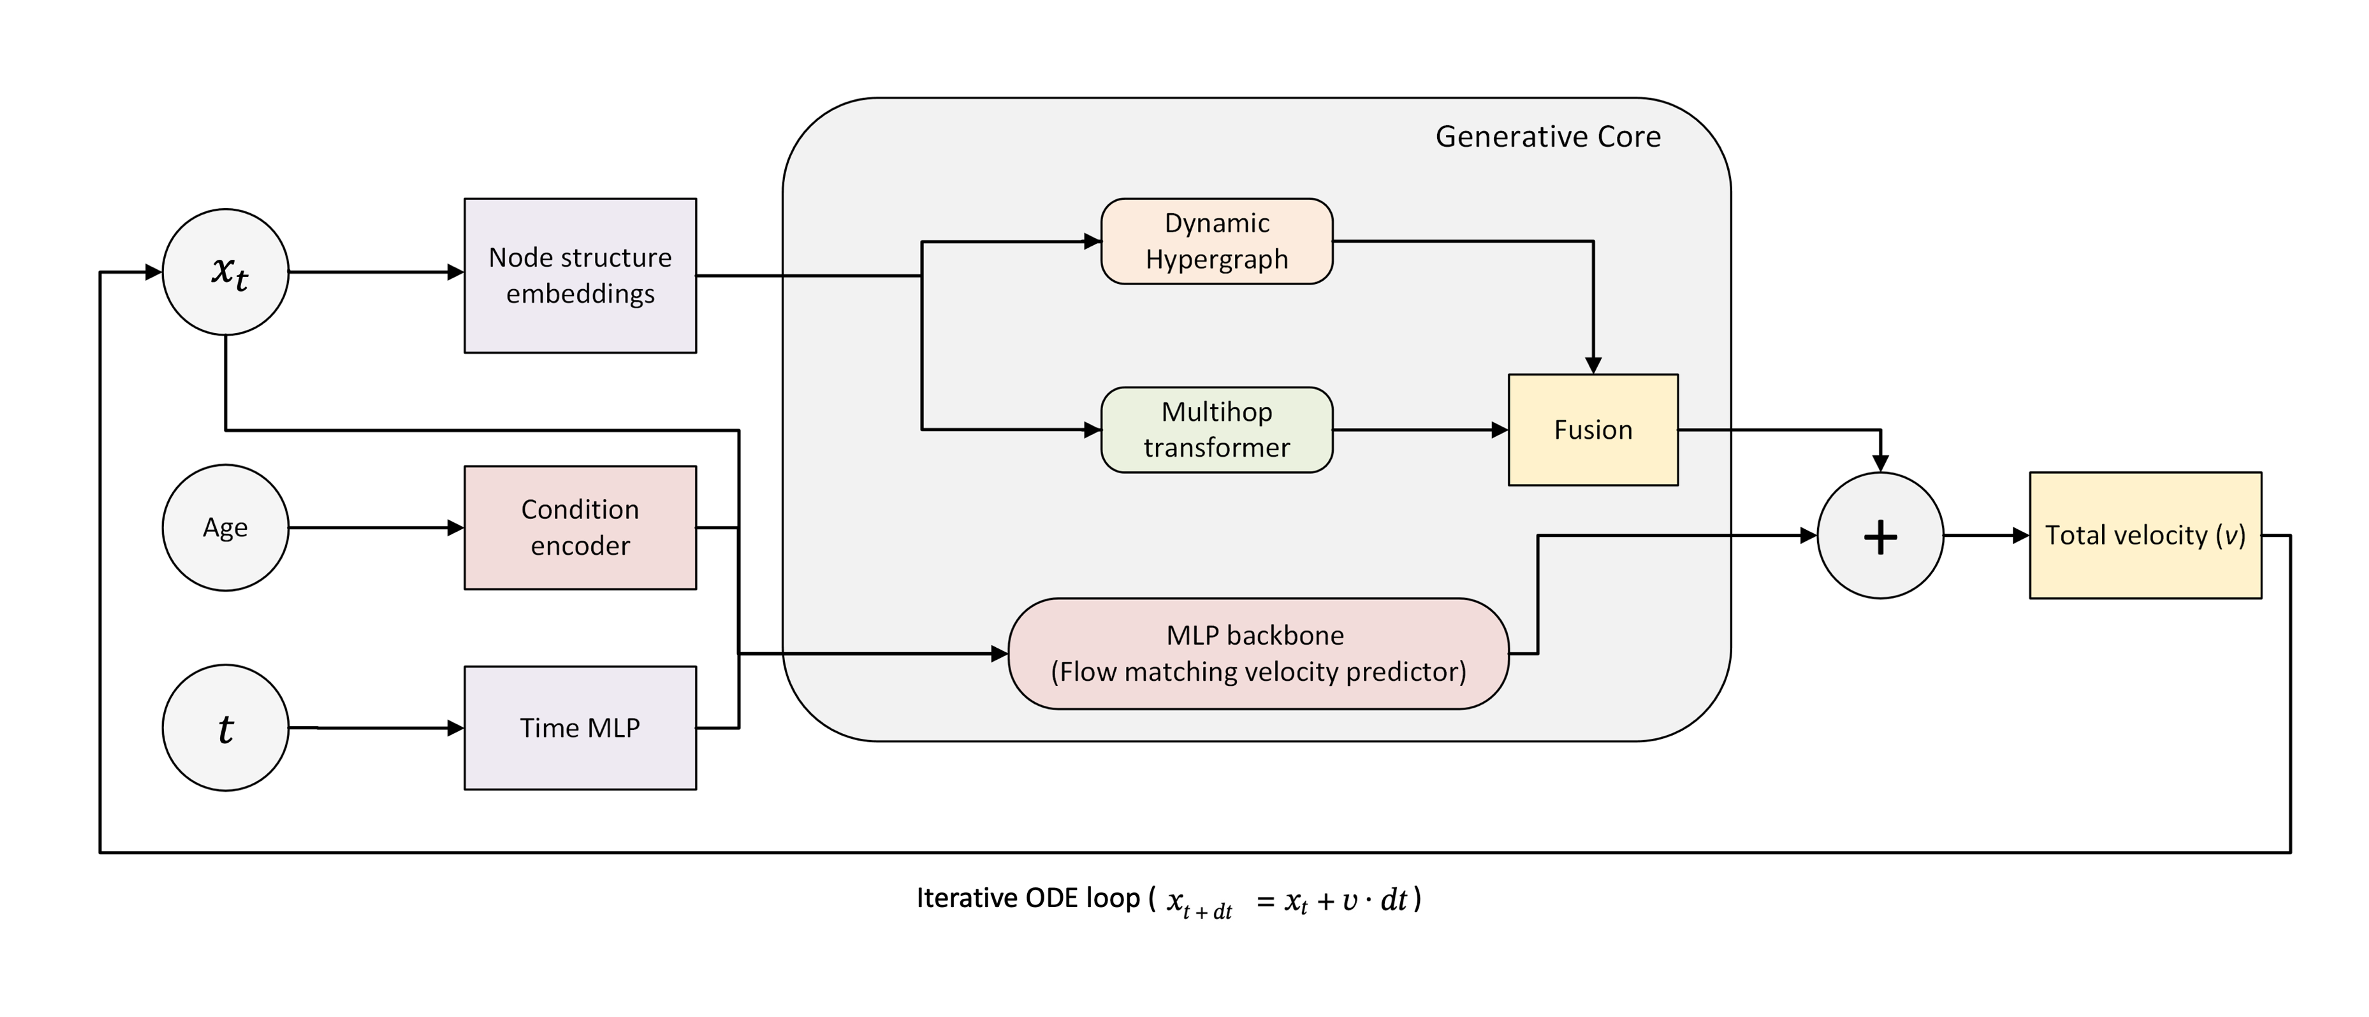
\includegraphics[width=\columnwidth]{figures/Model_diagram.png}
  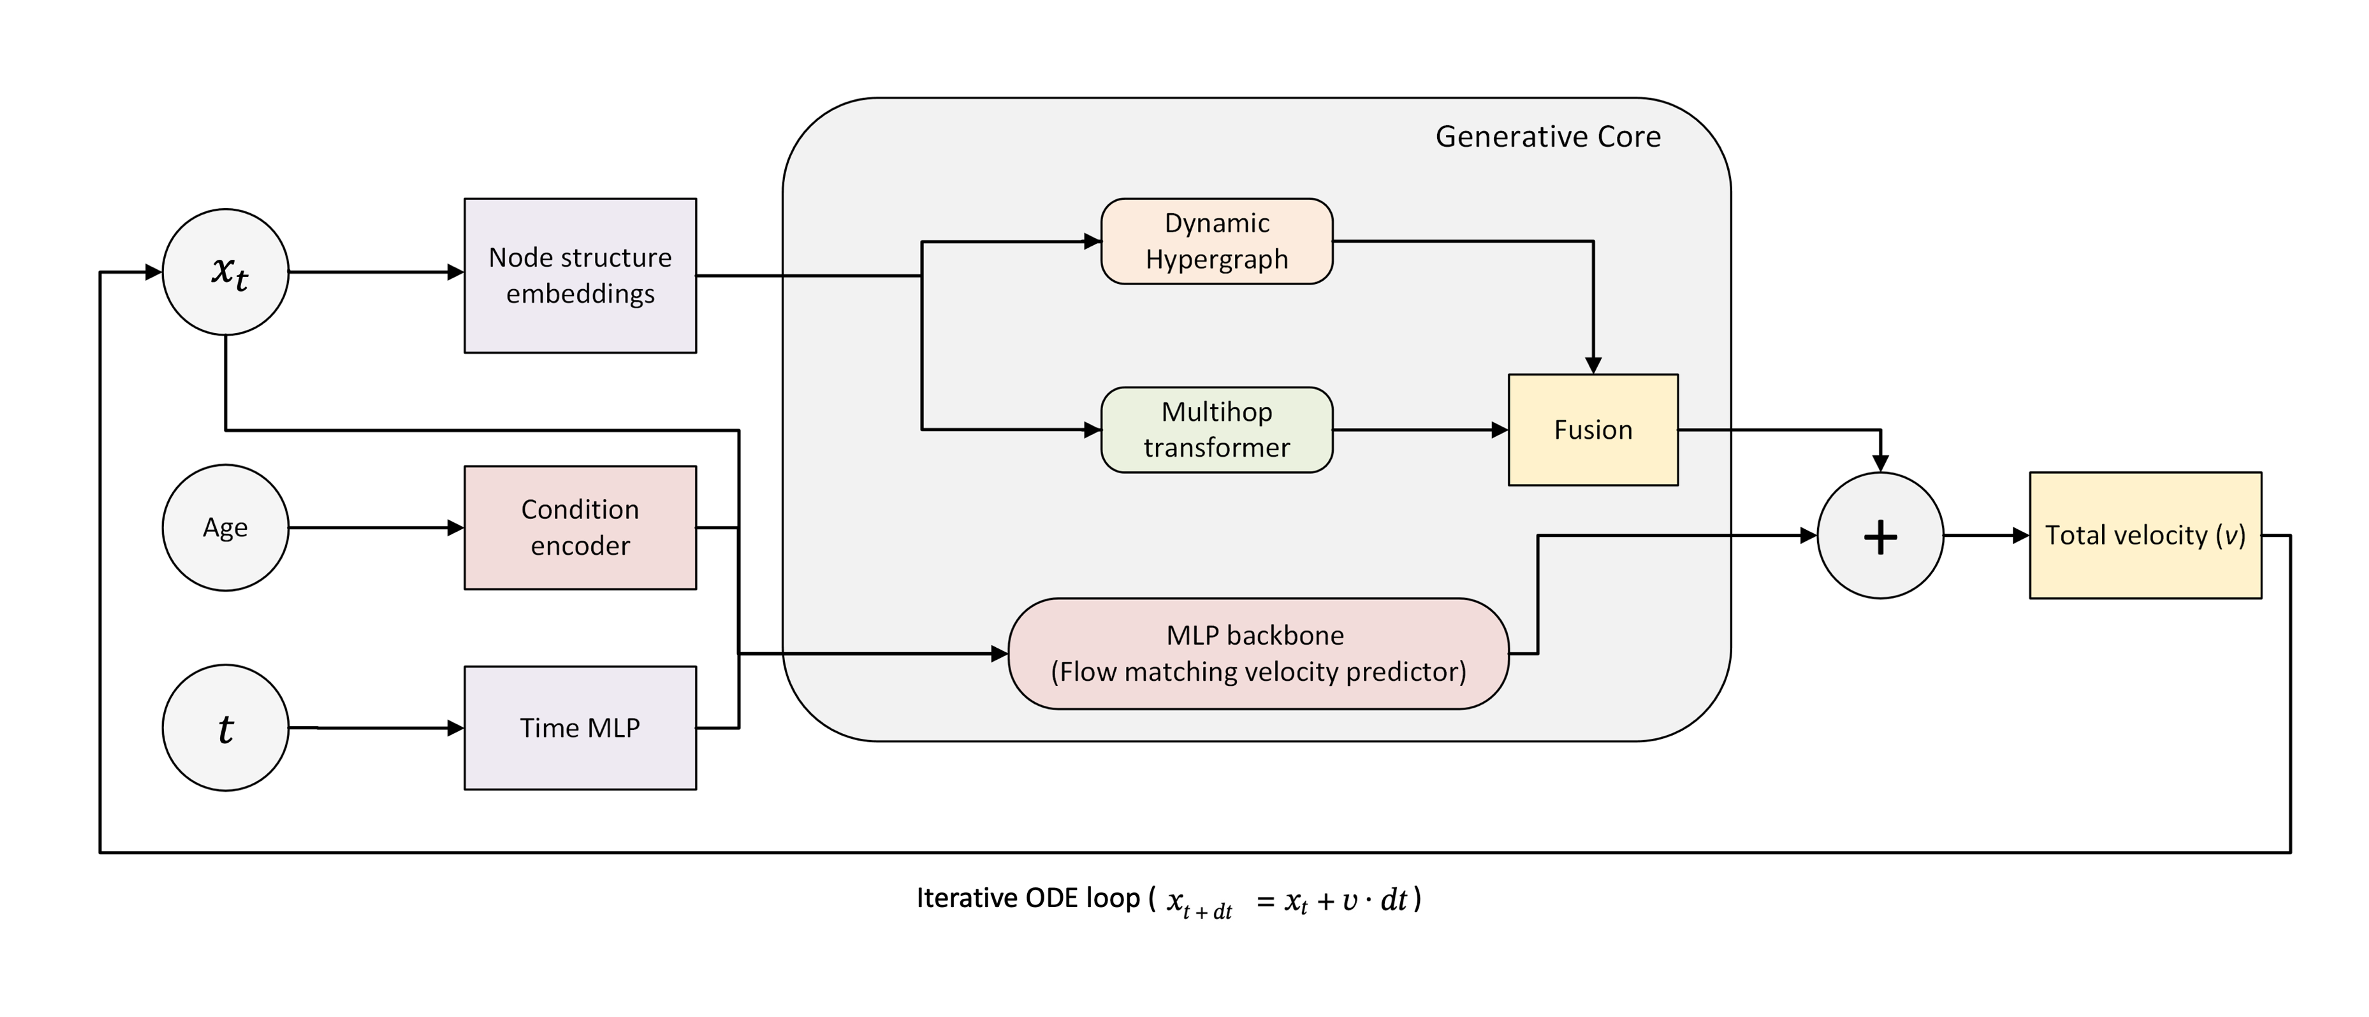
\includegraphics[width=0.99\textwidth]{figures/Model_diagram.png}
  \caption{Overview of proposed Generative Flow Matching training pipeline. The model consists of a standard flow-matching MLP backbone, conditioned with gestational age (GA). Structural information about the brain geometry is fed to parallel Dynamic Hypergraph, and Multihop Transformer streams which are fused in order to learn complex topological structures. These three components are combined to predict the total velocity ($v$) which is used to define a probability path between the noise distribution and the target brains through iterative ODE solving.}
  \label{fig:model}
\end{figure*}

% \subsection{Graph Representation}

\subsection{Dataset}
     We use data from the developing human connectome project (dHCP) which is a large-scale study into the human brain at the time of birth. (\cite{hughes2017dedicated}) processed by \cite{taoudi2022predicting} and available on their GitHub.
    This includes Diffusion Tensor Imaging (DTI) data from 520 newborn infants. Data was collected at term-normalized age, meaning that all infants were imaged shortly after their ``due date''. The age indicated is gestational age (GA), which is the number of weeks from conception to the date of birth.

    The brain structural connectome for each infant is encoded as a symmetric adjacency matrix $A_i \in \mathbb{R}^{n \times n}$,  where \textit{n} is the number of nodes, representing distinct regions in the brain. The entry $A_i[u, v]$ gives the strength of the connection between region $u$ and region $v$.
    
% \subsubsection{Dynamic Hypergraph}



        

\subsubsection{Node Features}
We initialize the node representations with a base embedding $e_i^{(0)}$ which combines the anatomical information about the corresponding brain region. This base node embedding is:
    \begin{equation}
        \begin{split}
            e_i^{(0)} = {} & \text{Emb}_{reg}(r_i) + \text{Emb}_{lobe}(l_i) + \text{Emb}_{surf}(s_i) \\
            & + \text{Emb}_{hemi}(h_i) + \text{MLP}_{coord}(x_i, y_i, z_i),
        \end{split}
    \end{equation}
where $r_i$, $l_i$, $s_i$ and $h_i$ are the region, lobe, surface, and hemispheres for each index, as defined by the brain parcellation atlas \cite{taoudi2022predicting}.
Coordinates represent the centroid of each brain region in the infant brain atlas that was used in the initial processing of the DTI data \cite{shi2011infant, schuh2018unbiased}.

While there is spatial information in these features, connectivity patterns arise from the relative dependences between nodes. Therefore, we add a multihop transformer layer, to attend to these embeddings in relation to each other. We fuse the information from the hypergraph and the transformer, in order to synthesize local and global topologies into a unified representation. 
         % initially, we embed each node with information relating to their physical location (\textit{i.e.} we provide X,Y,Z coordinates, lobe, hemisphere and surface), however these pieces of information are important relative to one another.


\subsubsection{Edge Features}
In the dataset, edges refer to physical connections between regions in the brain. Therefore, we treat edges as carriers that allow for informtion flow throughout the network. We include them in hyperedges alongside nodes to facilliate interation between and within hyperedges. We distinguish two conditions for edges in the hypergraph:
\begin{itemize}
    \item Reinforcement: These are edges that connect two nodes within the same hyperedge. The strength of the edge reinforces the structural cluster of the hyperedge.
    \item Bridges: These are edges that connect nodes in distinct hyperedges. We calculate the signal of these in order to inform the proximity between the latent clusters. This allows the model to understand the global relationship between the hyperedges.
\end{itemize}

\subsection{Hypergraph formation}

Features from nodes are passed to the dynamic hypergraph layer to explore communities within the brain structure. The model generates a membership matrix $H$ which allows grouping of nodes. We use a soft-assignment which allows for nodes to participate in multiple hyperedges, and this membership is recalculated at every graph state $x_t$. This allows the model to learn different patterns of connectivity as the state evolves. In order to facilitate the dynamic membership of nodes within hyperedges, we implement entropy loss with a dual-objective. We aim to balance the ``sharpness'' of communities, with the ``diversity''. This means that while we use a soft-assignment, we incentivize the model to decisively group nodes into hyperedges . However, we also push the model to prioritize diverse hyperedges across the full feature space instread of a few large non-specific group. Importantly, these hyperedges represent latent clusters not simply anatomical groupings, and which evolve with the graph state.
subsubsection{Soft assignment}

\subsubsection{more ideas to add}


\textbf{How H is computed 
}
\textbf{How H depends on graph state xt }

\textbf{How memberships are updated 
}
\textbf{Normalization constraints on membership  
}
\textbf{How H interactis with multihop and backbone 
}

\subsection{Generative model}
\subsubsection{Flow-matching}
We employ Conditional Flow Matching (CFM) \cite{lipman2023flowmatchinggenerativemodeling} to implicitly learn the mapping between Gaussian noise and the complex brain connectivity. This draws a linear probability path between the real data ($x_0$) and the noise distribution ($x_1$):

    \begin{equation}
        x_t = (1 - t)x_0 + t x_1, \quad t \in [0, 1].
    \end{equation}

From this path, the CFM learns a vector field ($v_\theta$), which is the derivative of the path with regards to $t$. This $v_\theta$ is optimised using Huber loss, due to the heavy-tailed distributions of the brain connectivity matrices. Overall, CFM is shown to provide stability during training, while allowing the dynamic hypergraph to explore the higher-order structure of the brain matrices.
At inference we predict the novel brain graphs at a certain condition value ($c$) by solving the system of first-order ODEs :

    \begin{equation}
        \frac{d\mathbf{x}}{dt} = v_\theta(\mathbf{x}_t, t, c) ,
    \end{equation}

    from $t=1$ to $t=0$, and where $c$ is gestational age (GA). We update the graph state, $x_t$, through the Euler method:

    \begin{equation}
        x_{t-dt}= x_t - v_\theta (x_t,t,c) \cdot dt .
    \end{equation}

By conditioning on GA, we are able to specify the target age, in order to generate age appropriate networks. In Figure \ref{fig:flow} we demonstrate the differing trajectories, starting from identical Gaussian noise.
In order to improve robustness of this learning, and encourage the model to learn the relative effect of biological maturity on structure, we use classifier-free guidance. This allows the model to learn both the conditioned ($v_c$) and unconditioned ($v_u$) structures simultaneously. 
   
\subsubsection{Biologically inspired losses}

The brain connectivity matrices show heavy-tailed distributions, where there are a small number of high-strength ``hubs'' and many weaker nodes and connections. These hubs are particularly important as a feature of the development. In order to ensure that this is not diluted, we apply Huber loss. This retains nuance required for the biological data, by applying quadratic MSE for small error values, and MAE linearity at higher values.


\subsection{Evaluation metrics}
To assess the topological fidelity and biological plausibility of the generated networks, we evaluate based on graph-theoretical metrics. This allows us to observe how well the model has reproduced complex network characteristics.

We split these into two categories to clearly demonstrate the scale that they are working on \cite{rubinov2010complex}:
\subsubsection{Global performance metrics} In this category we calculate the Global Efficiency, the Spectral Wasserstein Distance and the Value Wasserstein Distance of the network. These assess the overall alignment of the synthetic data with the real test set. Results are reported in Table \ref{tab:global_integration}
\begin{itemize}
    \item \textit{Global efficiency($E$)}: This gives a measure of how efficiently the network allows information exchange:
    \begin{equation}
        E = \frac{1}{n(n-1)} \sum_{i \neq j \in G} \frac{1}{d_{ij}} ,
    \end{equation}
     where $n$: The total number of nodes in the graph.$d_{ij}$: The shortest path length between node $i$ and node $j$ \cite{PhysRevLett.87.198701}.
     
    \item \textit{Spectral Wasserstein Distance ($W_{spec}$)}: Gives a distance between the eigenvalue distributions of the graph Laplacians ($L = D - A$):
    \begin{equation}
        W_{spec} = \frac{1}{n} \sum_{i=1}^{n} |\lambda_i^R - \lambda_i^S| ,
    \end{equation}
    where the sorted eigenvalues of real and synthetic Laplacian matrices are given by $\lambda^R$ and $\lambda^S$.
    
    \item \textit{Value Wasserstein Distance ($W_{val}$))}: This gives the distance between the two cumulative distribution functions of edge weights for real and synthetic data ($F_P$ and $F_Q$):
    \begin{equation}
        W_{val}(P, Q) = \int_{-\infty}^{\infty} |F_P(x) - F_Q(x)| dx ,
    \end{equation}
\end{itemize}
\subsubsection{Topological fidelity} These look more closely for specific patterns of connectivity that are commonly found in the human brain structural connectome \cite{sporns_human_2013}. We focus on characteristics that demonstrate the diverse range of biological connection patterns. Results are reported in Table \ref{tab:local_topology}
\begin{itemize}
    \item \textit{Clustering Coefficient ($C$)}: This indicates how densley connected neighbours are by observing how many triagles form within the network \cite{watts1998collective}:

    \begin{equation}
        C = \frac{1}{n} \sum_{v \in G} c_v ,
    \end{equation}
    where $c_v$ is the clustering coefficient for node $v$.
    
    \item \textit{Small-World Index ($\sigma$)}: This metric measures the tendency for all nodes to be connected to one another through a short number of ``hops'' \cite{humphries2008network}. This is a ratio of how clustered the network is, against how integrated the network is:

    \begin{equation}
        \sigma = \frac{C / C_{rand}}{L / L_{rand}} ,
    \end{equation}

    where $C_{rand}$ and $L_{rand}$ come from approximations of Erdős-Rényi graphs. These were:

    \begin{equation}
        C_{rand} \approx p = \frac{E}{N(N-1)/2} ,
    \end{equation}
    and 
    \begin{equation}
        L_{rand} \approx \frac{\ln(N)}{\ln(\langle k \rangle)}.
    \end{equation}
    
    
    \item \textit{Rich Club Coefficient ($\Phi$)}: This quantifies the tendency for hubs (highly connected nodes) to connect with each other:

    \begin{equation}
        \Phi(k) = \frac{2 E_{>k}}{N_{>k}(N_{>k}-1)} \quad \implies \quad \Phi_{norm}(k) = \frac{\Phi(k)}{\Phi_{rand}(k)},
    \end{equation}

    where $k$ is degree threshold \cite{van2011rich, colizza2006detecting}.
    
\end{itemize}
    


\section{Experiments}
\subsection{Experimental setup}
\subsubsection{Stratified split}

        To ensure the representation of development spectrum, we implemented a stratified three-way split (80/10/10). We based this on the clinical definitions of preterm and term ($GA < 37$ and $GA \geq 37$). This allowed us to ensure that each contained an equivalent distribution of the two main developmental classifications. This also ensured that the miniority class (preterm) were appropriately distributed throughout all three splits. 

        \textbf{Add about cross validation folds}
        \textbf{Also add about hold one out age generation}
        \textbf{consider generating across multiple seeds}
        

\subsection{Results}



\subsection{Biological correspondance of hyperedges}

We can demonstrate the learning pattern of the Conditional Flow Matching by decomposing the learned flow trajectories between the noise and real brain data. This can be demonstrated through PCA analysis. We can show the effect of conditioning by starting from identical Gaussian, and then projecting the paths to the data from each age condition. We demonstrate here with high and low GA values which is demonstrated in Figure \ref{fig:flow}.
 \begin{figure}
    \centering
    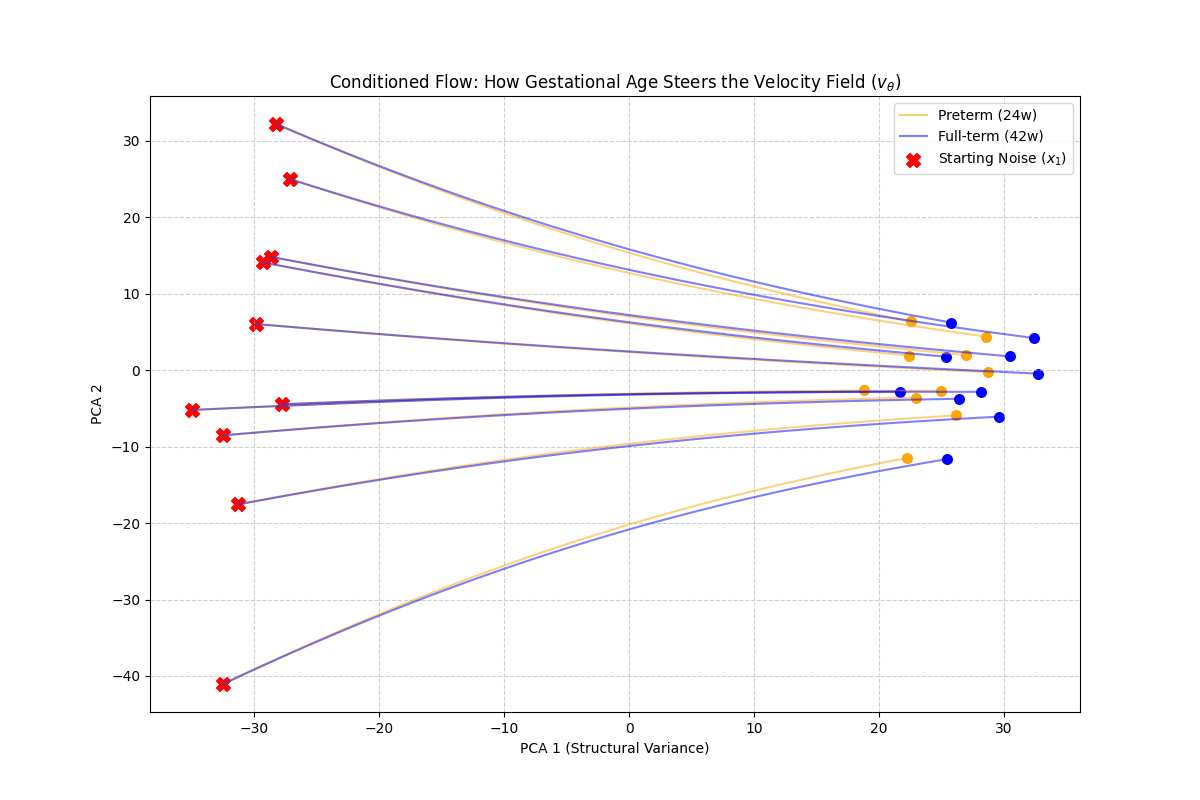
\includegraphics[width=1\linewidth]{figures/flow_conditioned.png}
    \caption{Plot showing a decomposition of how the conditioning affects the flow. Yellow points indicate the end points for preterm infants, while blue indicate end points for term infants. Both cases start from the same Gaussian noise distribution.}
    \label{fig:flow}
\end{figure}

            % \item we need to ensure that the graphs are not simply averaging. therefore we can correlate the GA with each metric, and check that the model can understand maturation
            % \item despite the binary split categories for the train/val/test, we are able to demonstrate a positive slope which is in line with the literature. this is actually better than the real test set due to a few reasons. firstly the test set was very small, secondly it was categorically defined. We show that while the ages within the preterm/term groups are noisy, the model interpolates a smooth maturation line using the Flow matching. 
            % In order to test this we check the results by decoupling GA from the real and synthetic data, and check the difference between the results and the real coupled gestational results. 

            % We present 3 types of comparison
            % BaselineVal (Real) vs Val (Real) Mean Absolute Error Biological variance limits. 
            % FidelitySyn vs Test (Real) Mean Absolute Error Model accuracy/precision.
\begin{figure*}[h]]
    \centering
    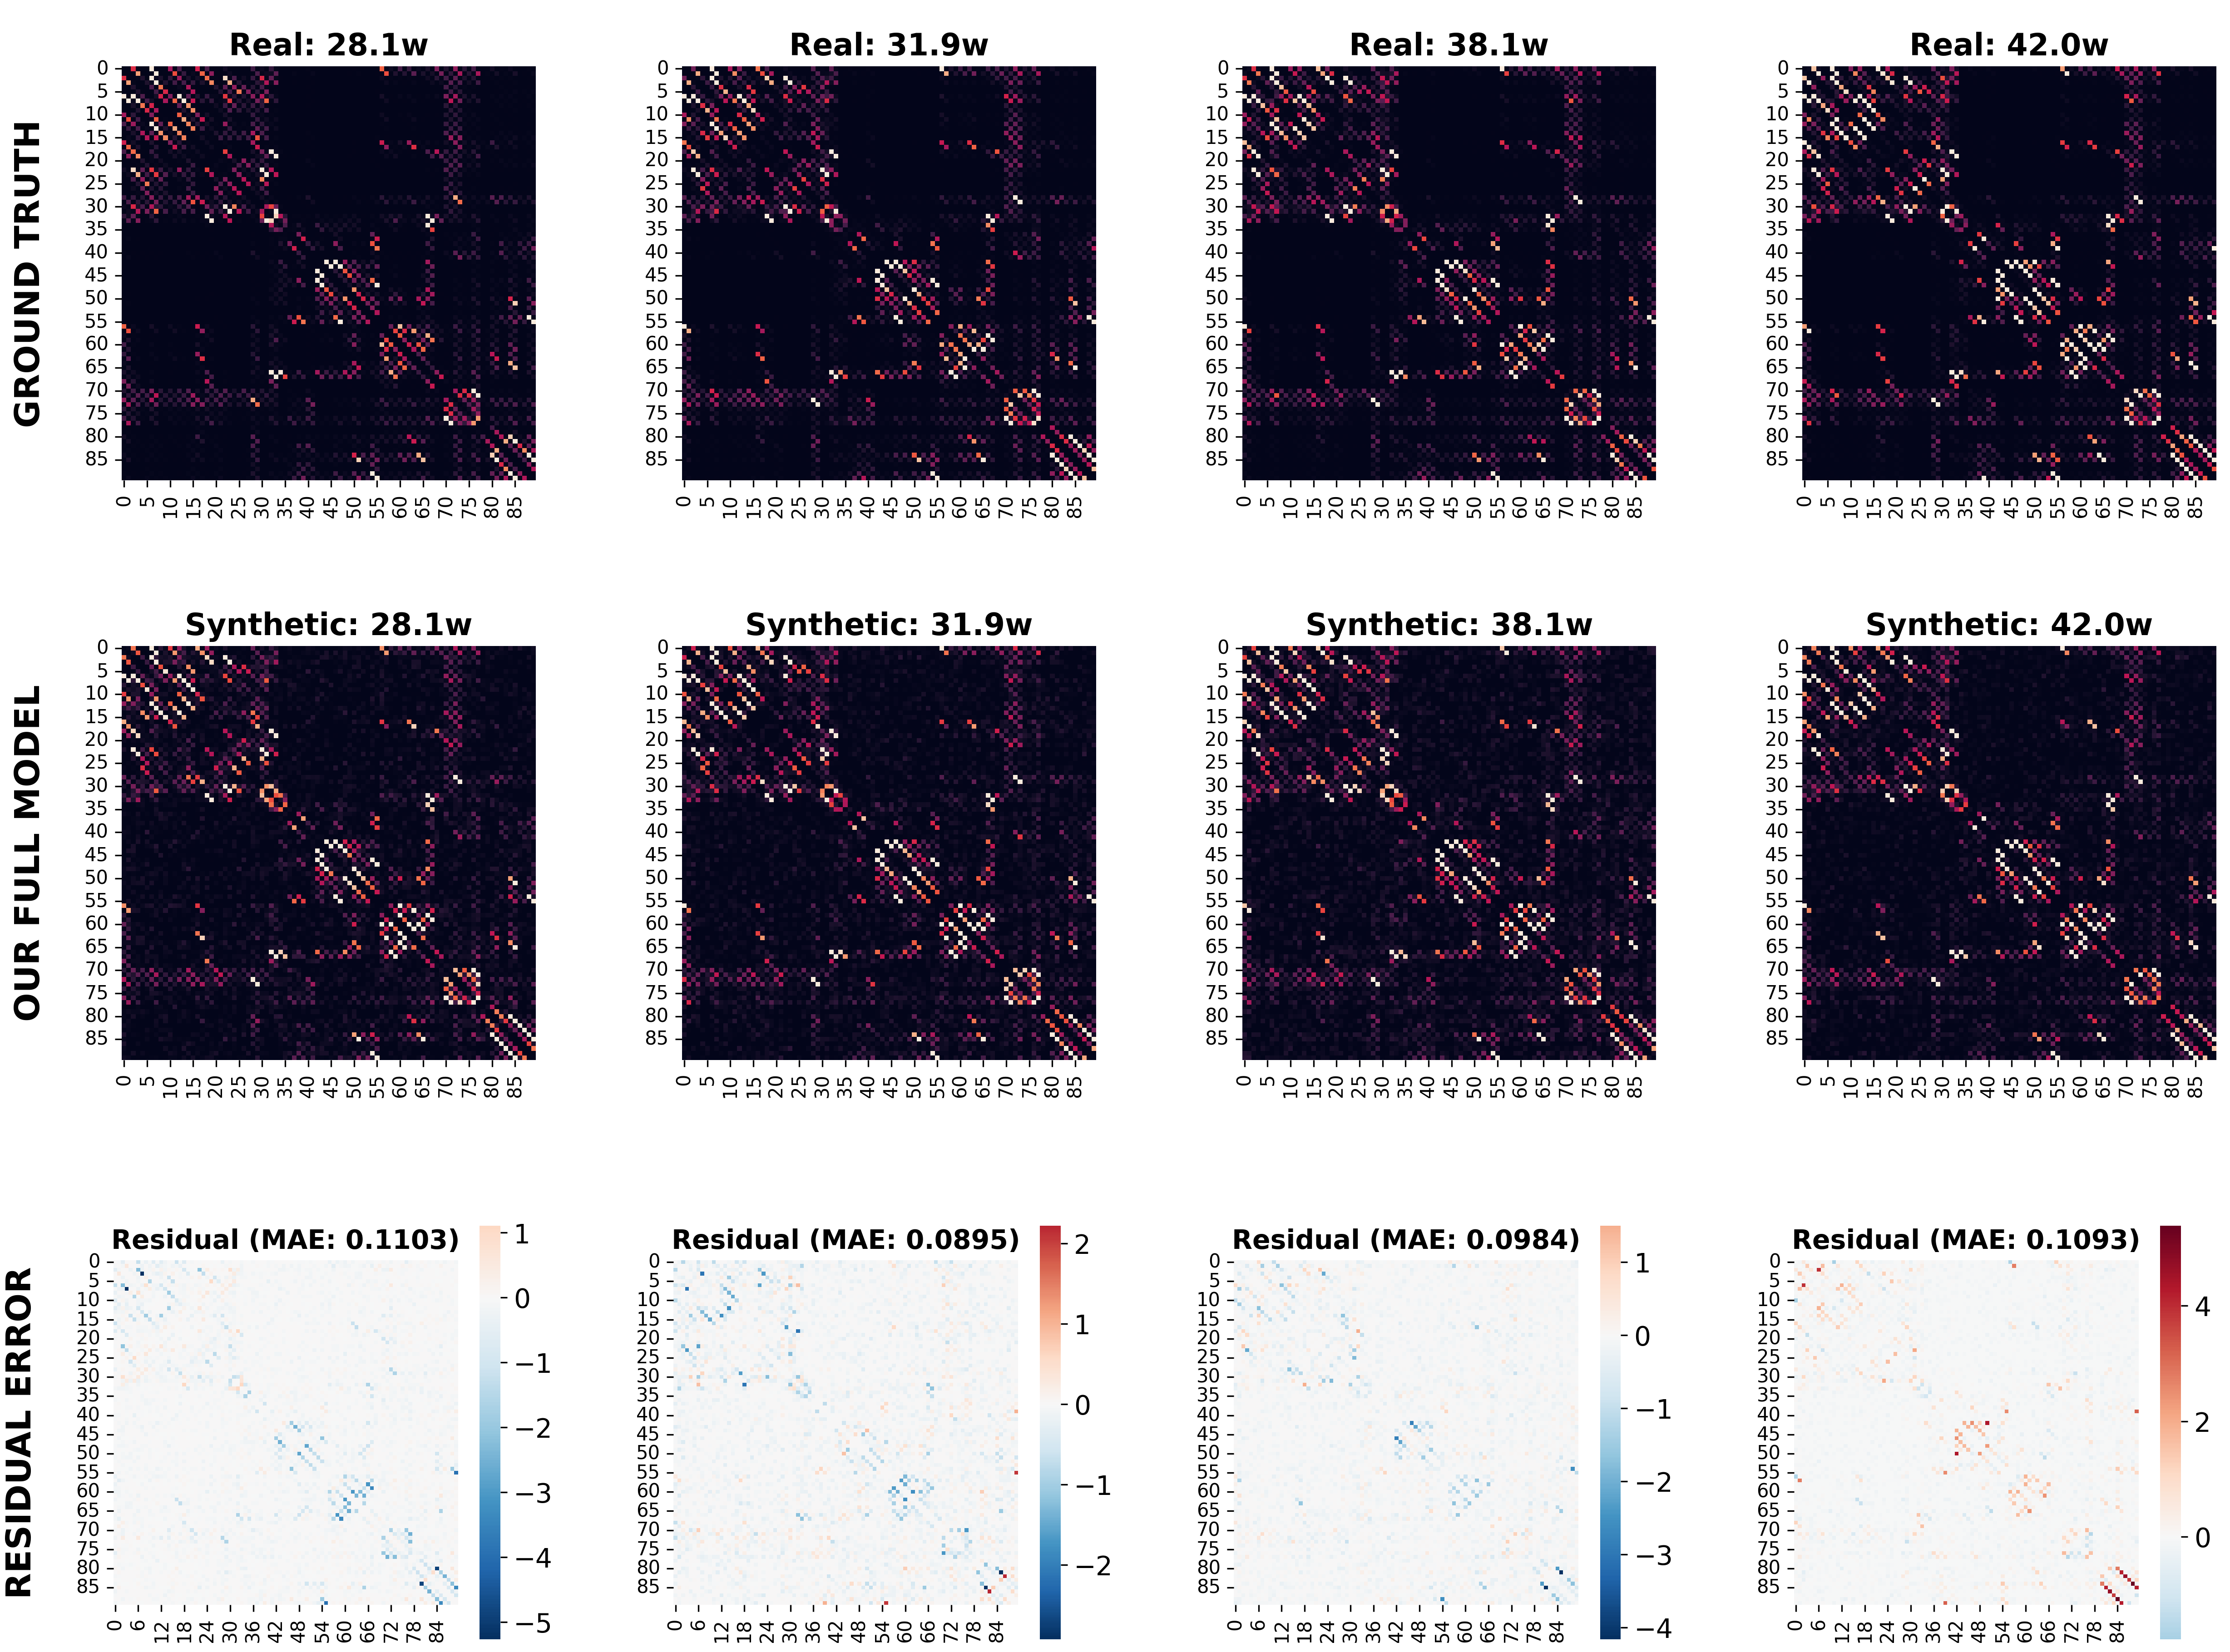
\includegraphics[width=1\linewidth]{figures/Maturation_Fidelity_Grid.png}
    \caption{Generative performance across GA spectrum. The figure displays ground truth (top), synthetic connectomes (middle) and comparison of residual error (bottom).}
    \label{fig:maturation}
\end{figure*}



\subsubsection{Competitor models}

In order to assess the efficacy of the proposed model, we compare with re-implementations of the models that were, to the best of our knowledge, closest to the aim. Therefore, we implement two alternatives, first a CVAE model reproduced from \cite{liu_deep_2025} and second a more traditional geometric generative model from \cite{betzel_generative_2016}. Due to the nature of the model, \cite{betzel_generative_2016} does not have a mechanism for modeling specific gestational ages, therefore this model is excluded from the gestational comparison metrics.

For a further comparison, we construct a baseline Denoising Diffusion Probabilistic Model (DDPM) based on the formulation from \citet{ho2020denoising}.

In all comparisons, we use the same train/val/test indices, to ensure fair comparison. Moreover, we prompt each model to generate ``datasets'' with the same number of cases, and the same matched GA split as the test set. For a baseline, we compare the differences in distribution between the test and validation sets, which gives an indication of both how well the selected indices are representative but also of the natural expected variance within the real data. 



\subsubsection{Ablations}

We run a selection of ablation studies in order to observe the effect of each component on the resulting networks. The three ablations are: 1. Without hypergraph layer; 2. Without multihop transformer; 3. Without hypergraph or multihop. The results are displayed in Table \ref{tab:abl_loss}.
In addition, we compare the test set with the validation set (Table \ref{tab:consist}), in order to ensure representativeness of the sample beyond age.

% \begin{table}[h]
% \caption{Comparison of models using topological graph metrics}
% \label{tab: comparison}
% \centering
% \begin{tabular}{lclll}
% \toprule
%                & \multicolumn{4}{c}{\textbf{Graph Theory Metrics (Synthetic vs. Real)}}                    \\ \cline{2-5} 
% \textbf{Model Name} & \textbf{Eff. Error} & \multicolumn{1}{c}{\textbf{Clust. Error}} & \multicolumn{1}{c}{\textbf{Path Length}} & \multicolumn{1}{c}{\textbf{Deg. Dist.}} \\ \hline
% Ours           & \multicolumn{1}{l}{} &                      &                      &                      \\
% Geometric \cite{betzel_generative_2016} &                      & \multicolumn{1}{c}{} & \multicolumn{1}{c}{} & \multicolumn{1}{c}{} \\
% CVAE \cite{liu_deep_2025}   & \multicolumn{1}{l}{} &                      &                      &  
% \bottomrule
% \multicolumn{5}{l}{\footnotesize \textit{Note: Values represent the mean absolute error (MAE) relative to the ground truth.}}
% \end{tabular}
% \end{table}


% \begin{table}[h]
% \caption{Model Comparison: Global Performance
% \textit{N.B. comparisons for $W_{spec}$ and $W_{val}$ represent distances between synthetic and real distributions, therefore cannot be computed for the ground truth (test) dataset. Ground truth row represents raw metric means, while other rows represent MAE. }}
% \label{tab:global_integration}
% \centering
% \begin{tabular}{lccc}
% \toprule
% \textbf{Model Name} & \textbf{$E$}& \textbf{$W_{spec}$}  &$W_{val}$ \\
%  Ground truth& 0.3879&  ---&---\\ \hline
% \textbf{Ours (Full Model)} & 0.0120& 0.7535 & 0.0568\\
% \midrule
% No Hypergraph & 0.1891& 1.1568&0.1395\\
% No Multihop & 0.0260& 0.8117& 0.0671\\
% Baseline MLP & 0.1883 & 1.2945 & 0.1429\\
 
%  \midrule
% Geometric \cite{betzel_generative_2016} & 0.0283& 3.2138 &0.1351\\
% CVAE \cite{liu_deep_2025} & 0.0154& 0.9029 &0.0326\\
% \bottomrule
% \end{tabular}
% \end{table}
\begin{table}[h]
\caption{Model Comparison: Global Performance. 
\textit{N.B.} $W_{spec}$ and $W_{val}$ represent distributional distances and are null for the ground truth. Ground truth row represents raw metric means; other rows represent MAE (Relative Error \%).}
\label{tab:global_integration}
\centering
\begin{tabular}{lccc}
\toprule
\textbf{Model Name} & \textbf{$E$ (MAE)} & \textbf{$W_{spec}$} & \textbf{$W_{val}$} \\ 
\midrule
Ground Truth (Test) & 0.3879 & --- & --- \\ 
\midrule
\textbf{Ours (Full Model)} & \textbf{0.0120 (3.1\%)} & \textbf{0.7535} & 0.0568 \\
\midrule
No Hypergraph & 0.1891 (48.7\%) & 1.1568 & 0.1395 \\
No Multihop & 0.0260 (6.7\%) & 0.8117 & 0.0671 \\
Baseline MLP & 0.1883 (48.5\%) & 1.2945 & 0.1429 \\
\midrule
Geometric \cite{betzel_generative_2016} & 0.0283 (7.3\%) & 3.2138 & 0.1351 \\
CVAE \cite{liu_deep_2025} & 0.0154 (4.0\%) & 0.9029 & \textbf{0.0326} \\
\bottomrule
\end{tabular}
\end{table}

% \begin{table}[h]
% \caption{Model Comparison: Topology
% \textit{N.B. Ground truth row represents raw metric means, while other rows represent MAE.}}
% \label{tab:local_topology}
% \centering
% \renewcommand{\arraystretch}{1.3}
% \begin{tabular}{lccc}
% \toprule
% % \textbf{Model Name} & \textbf{Clust. Error} & \textbf{Sigma Error} & \textbf{Value WD} & \textbf{Rich club}\\ \hline
% % \toprule
% \textbf{Model Name} & \shortstack{\textbf{Clust.} \\ \textbf{Error}} & \shortstack{\textbf{Sigma} \\ \textbf{Error}} & \shortstack{\textbf{Rich} \\ \textbf{Club}} \\
%  Ground truth& 0.5462& 4.3499&\\ 
% \midrule
% \textbf{Ours (Full Model)} & \textbf{0.0238} & \textbf{0.2497} &0.0842\\
% \midrule
%  No Hypergraph & 0.2899& 3.1170&\\
%  No Multihop & 0.0380& 0.5802&\\
%  Baseline MLP & 0.2879& 3.1077&\\
%  \midrule
% Geometric \cite{betzel_generative_2016} & 0.0299 & 5.9183 & \\
% CVAE \cite{liu_deep_2025} & 0.0249 & 0.4453 &\\
% \bottomrule
% \end{tabular}
% \end{table}

\begin{table}[h]
\caption{Model Comparison: Topological Fidelity. 
\textit{N.B.} Ground truth row represents raw metric means; other rows represent MAE (Relative Error \%).}
\label{tab:local_topology}
\centering
\renewcommand{\arraystretch}{1.3}
\begin{tabular}{lccc}
\toprule
\textbf{Model Name} & \shortstack{\textbf{Clust.} \\ \textbf{Error}} & \shortstack{\textbf{Sigma} \\ \textbf{Error}} & \shortstack{\textbf{Rich} \\ \textbf{Club} }(Rel. \%)\\ 
\midrule
Ground Truth (Test) & 0.546 & 4.350 & 1.040\\ 
\midrule
\textbf{Ours (Full Model)} & \textbf{0.024 (4.3\%)} & \textbf{0.250 (5.7\%)} & 0.084 (8.1\%)\\
\midrule
No Hypergraph & 0.290 (53.1\%) & 3.117 (71.7\%) & 0.217 (20.8\%)\\
No Multihop & 0.038 (6.9\%) & 0.580 (13.3\%) & 0.171 (16.4\%)\\
Baseline MLP & 0.288 (52.7\%) & 3.108 (71.4\%) & 0.221 (21.2\%)\\
\midrule
Geometric \cite{betzel_generative_2016} & 0.030 (5.5\%) & 5.918 (136.1\%) & 0.493 (47.3\%)\\
CVAE \cite{liu_deep_2025} & 0.025 (4.5\%) & 0.445 (10.2\%) & 0.197 (18.9\%)\\
\bottomrule
\end{tabular}
\end{table}

\begin{table}[h]
\caption{Ablation study of our model testing the impact of different architectural components. The table highlights accuracy on validation loss.}
\label{tab:abl_loss}
\centering
\begin{tabular}{l cc c}
\toprule
& \multicolumn{2}{c}{Architecture} & \\
    \cmidrule(r){2-3}
    Model Name & Transformer & Hypergraph & Best Validation Loss \\
\midrule
Full         & \checkmark  & \checkmark & \textbf{0.148}\\
Multihop     & \checkmark  & $\times$   & 0.432\\
Hypergraph   & $\times$    & \checkmark & 0.194\\
Baseline MLP & $\times$    & $\times$   & 0.434\\
\bottomrule

\end{tabular}
\end{table}

\begin{table}[]
\caption{Consistency between validation and test set. This demonstrates that while both splits are small ($n=53$) they include similar distributions for each graph network feature.}
\label{tab:consist}
\centering
\renewcommand{\arraystretch}{1.3}
\begin{tabular}{@{}lcc@{}}
\toprule
\textbf{Metric} & \shortstack{\textbf{Variance} \\ \textbf{($p$-value)}} & \shortstack{\textbf{Mean} \\ \textbf{($p$-value)}} \\
\midrule
Clustering Coefficient ($C$)     & 0.178 & 0.175 \\
Global Efficiency ($E$)          & 0.165 & 0.355 \\
Characteristic Path Length ($L$) & 0.174 & 0.432 \\
Small-Worldness ($\sigma$)       & 0.956 & 0.495 \\ \hline
\multicolumn{3}{l}{\footnotesize \textit{Note: High p-values indicate no significant distributional shift.}}
\bottomrule
\end{tabular}
\end{table}


\subsection{Global performance}
Results from Table \ref{tab:global_integration}
show that our full model achieves the best scores overall for global performance metrics. From this table we can see that our full model outperforms all comparison models on all metrics, with the exception of $W_{val}$ where we are second to the CVAE. This suggests that while the CVAE is able to reproduce appropriate edge strengths globaly, it does so at the expense of structural organization. Figure \ref{fig:maturation} demonstrates that the Flow Matching layer is able to appropriately generate a range of different ages across GA. In the residual heatmaps, areas that are near-white represent near-perfect reconstruction, while faint red or blue spots highlight where the model either slightly overestimates or underestimates connection strength. This therefore demonstrates a high similarity between the age matched cases.

\subsection{Topolocial fidelity}
From Table \ref{tab:local_topology} we demonstrate that our approach can identify and reproduce complex network features which are characteristics of the real brain data. With our full model, we achieve the lowest error across all metrics indicating that the generative model reproduces the density and efficiency in line with real data. Moreover, the $\sigma$ results demonstrate ``small-world'' connectivity, which is a key feature of human brain connectomes \cite{humphries2008network} as it illustrates the balance between local clustering and global integration. Similarly, ``rich club'' results are also important, as they have been implicated as critical features of neurodevelopment, and particular markers in preterm birth \cite{bauer2017nonlinear, karolis2016reinforcement}.



\subsection{Ablations}
In Table \ref{tab:abl_loss} we evaluate the impact of each component of the model on validation performance. From this we see that the full model performs the best, followed by the model with no multihop transformer. This suggests the dynamic hypergraph layer is the most impactful component, which can be improved by including the transformer layer.

This is further supported by the Tables \ref{tab:global_integration} and \ref{tab:local_topology}, which demonstrates that on both global and local scales, the removal of the hypergraph leads to collapse in fidelity. This reinforces the biological hypothesis that higher-order relationships are the key to gestational development of the brain structural connectome. 
While the model with no multihop transformer generally performs well across metrics, there is an increased error particularly for the small-worldness, which suggests that the transformer still provides insight into how local clusters become globally integrated.

\section{Use case: Binary classification}
In order to test usability of the generated data, we re-implement a fuzzy classifier based on prior work \cite{birch2025exploring} which found that due to individual differences in biology, and in estimating GA, it can be difficult to define exactly which infants are premature \cite{birch2025exploring, jukic2013length, moutquin2003classification, engle2006recommendation, karnati2020late} when using a hard decision boundary ($GA < 37$). We therefore use the fuzzy boundary, and attempt to classify our synthetic data into preterm and term, training only on the real dataset. We use the same train/test/validation indices for the classification training, and employ a logistic regression (LR) model. For each of the models, we generate a dataset with the same age distributions as the real test set.

In generating our data, we conditioned on continuous GA, and therefore classifying the binary ``preterm'' and ``term'' indicates that the model has appropriately generated realistic developmental trajectories. 
% This use case is important, as it demonstrates the efficacy of the model. A model could produce something that looks realistic, but lacks the specific connectivity patterns found in real human development. Even when some graph metrics match. Therefore, we look at the case of preterm birth, where evidence can show that there are distinct differences between brain structural connectivity of preterm and full-term born infants at the time of birth. The model has the ability to generate based on a specific number of weeks GA, however, it is not specifically told whether there should be differences among these different age ranges. If the model is able to reproduce the real connectivity patterns, then it gives evidence that the model has been able to implicitly learn the representations of each of these classes, without being specifically conditioned on preterm or term class.
% To do this, we re-implement the fuzzy classifier \cite{birch2025exploring} to classify preterm and term.

\begin{table}[t]
\caption{Comparison of classification for preterm and term across real and synthetic datasets.}
\label{tab:classif}
\centering
\begin{tabular}{llcccc}
    \toprule
\textbf{Data}      & \textbf{Class}   & \textbf{Precision} & \textbf{Recall} & \textbf{F1}   & \textbf{Support (N)} \\
Real      & Preterm & 0.75      & 0.55   & 0.63 & 11     \\
          & Term    & 0.89      & 0.95   & 0.92 & 42     \\
          & Overall & 0.86      & 0.87   & 0.86 & 53     \\
\midrule
\textbf{Ours} & \textbf{Preterm} & 0.80      & 0.36   & 0.50 & 11     \\
          & \textbf{Term}    & 0.85      & 0.98   & 0.91 & 42     \\
          & \textbf{Overall} & 0.84      & 0.85   & 0.83 & 53     \\
\midrule
CVAE      & Preterm & 0.00      & 0.00   & 0.00 & 11     \\
          & Term    & 0.79      & 0.98   & 0.87 & 42     \\
          & Overall & 0.63      & 0.77   & 0.69 & 53    
\bottomrule
\end{tabular}
\end{table}






New tables here

















The results in Table \ref{tab:classif} demonstrate that the real test set can be classified with high precision and recall between classes. In contrast, the model was unable to identify any preterm cases in the CVAE dataset. On the other hand, when classifying data from our model, we achieved high precision of 80\% for the preterm class, and 85\% for term. This closely mirrors the results from the real dataset. Moreover, our model achieves ROC-AUC of 0.67, compared with the real data ROC-AUC of 0.84. However, the CVAE model, achieves only 0.49. 


\textbf{Moreover, when trained on a combined synthetic + real dataset, we increase the recall for preterm minority cases for the real data test set. } This is done through bootstrapped validation on the same unseen real data. 

\section{Future work and conclusion}
While our model produces state-of-the-art generations, the recall between preterm and term classes is still not ideal. Future work should focus on further mitigating the bias towards the majority class, in order to fully take advantage of the model's ability to generate networks across the full gestational range. While the model is demonstrating ability to reproduce preterm brain differences, in order to use the model for clinical outcome prediction, future work should incorporate longitudinal data.

In this paper, we assessed the sufficiency and plausibility of generating synthetic brain networks for infants based on their time of birth (GA). Previous works have relied on static reconstructions of real data, or purely statistical generation methods, where GA cannot be modeled. In our method, we introduced a model which is capable of generating brain connectivity as a continuous trajectory. This provides a platform for interpolating between GAs where there is data sparsity. 
Moreover, our model is able to implicitly learn higher-order structure as a function of gestational development. We test the appropriateness of our data, through a combination of biologically inspired losses, statistical metrics, and neurobiological graph-based metrics. In addition, we consider these in terms of trajectories. Our results demonstrate that the architecture can successfully learn and reproduce the brain's capacity for self-organization on local and global levels. Ultimately we demonstrate how the complex motifs of the human brain connectome can be captured through Conditional Flow Matching and learned higher-order structural priors. This offers a framework for modeling and exploring the differences at continuous stages of gestational development.


\section{Limitations and Ethical Considerations}
When working with the human data, it is important to ensure that individual participants cannot be reidentified. We have no information about the specific participants identities, and all infants are assigned index identifiers purely for the case of consistency in training. 
 Data were provided by the developing Human Connectome Project, KCL-Imperial-Oxford Consortium funded by the European Research Council under the European Union Seventh Framework Programme (FP/2007-2013) / ERC Grant Agreement no. [319456]. We are grateful to the families who generously supported this trial.


In the preparation of this manuscript, we utilized generative AI tools to enhance the research writing quality, adhering to the principles of responsible and transparent use. 

All AI-generated suggestions for text and structure were critically
reviewed, edited, and ultimately approved by the human
authors to ensure they accurately reflect our research contributions
and scientific voice. The core ideas, experimental methodology,
analysis, and conclusions presented in this paper are entirely the
work of the human authors.

\bibliographystyle{ACM-Reference-Format}
\bibliography{References_kdd}

% \section{Introduction}
\end{document}
